\documentclass[11pt]{report}
\usepackage[letterpaper, total={6.5in, 10in}]{geometry}
%\usepackage{fancyhdr}
%\pagestyle{fancy}
\usepackage{amsmath, amsthm, mathpazo, epic, eepic, color, array}
\usepackage{amssymb}
%\usepackage{graphicx}
\usepackage{cancel}
\usepackage{pgfplots}
\usepackage{multicol}
\pgfplotsset{compat=1.13}
\usepackage{etoolbox}
\makeatletter
\patchcmd{\chapter}{\if@openright\cleardoublepage\else\clearpage\fi}{}{}{}
\makeatother
\usepackage{hyperref}

\usepackage{enumerate}
\usepackage{enumitem}

\usepackage{tikz}
\usetikzlibrary{positioning,chains,fit,shapes,calc,arrows,patterns}
\usepackage{tkz-graph}
\usetikzlibrary{arrows, petri, topaths}
\usepackage{tkz-berge}
\usepackage[all]{xy}
\usepackage{textcomp}

\newboolean{colorprint}
\setboolean{colorprint}{true}
%\setboolean{colorprint}{false}

\ifthenelse{\boolean{colorprint}}{%
\newcommand{\colorone}{blue}
\newcommand{\colortwo}{red}
\newcommand{\coloronefill}{blue!15!white}
\newcommand{\colortwofill}{red!15!white}
\newcommand{\colormapone}{rgb=(.4,.4,1); rgb=(.8,.8,1)}
\newcommand{\colormaptwo}{rgb=(1,.4,.4); rgb=(1,.8,.8)}
\newcommand{\colormapplaneone}{rgb=(.7,.7,1); rgb=(.9,.9,1)}
\definecolor{colormaponebottom}{rgb}{.4,.4,1}
\definecolor{colormaponetop}{rgb}{.8,.8,1}
\definecolor{colormaptwobottom}{rgb}{1,.4,.4}
\definecolor{colormaptwotop}{rgb}{1,.8,.8}
}% ends color
{% not color
\newcommand{\colorone}{black}
\newcommand{\colortwo}{black!50!white}
\newcommand{\coloronefill}{black!15!white}
\newcommand{\colortwofill}{black!05!white}
\newcommand{\colormapone}{rgb=(.4,.4,.4); rgb=(.7,.7,.7)}
\newcommand{\colormaptwo}{rgb=(.6,.6,.6); rgb=(.9,.9,.9)}
\newcommand{\colormapplaneone}{rgb=(.8,.8,.8); rgb=(.95,.95,.95)}
\definecolor{colormaponebottom}{rgb}{.4,.4,.4}
\definecolor{colormaponetop}{rgb}{.7,.7,.7}
\definecolor{colormaptwobottom}{rgb}{.6,.6,.6}
\definecolor{colormaptwotop}{rgb}{.9,.9,.9}
}%

\newlength\tindent
\setlength{\tindent}{\parindent}
\setlength{\parindent}{0pt}
\renewcommand{\indent}{\hspace*{\tindent}}

\pgfplotsset{my style/.append style={axis x line=middle, axis y line=
middle, xlabel={$x$}, ylabel={$y$}, axis equal }}

\pgfplotsset{compat=1.13}

\usepackage[normalem]{ulem}

\begin{document}

{\bf Chapter 2: Derivatives}\\

%%%%%%%%%%%%%%%%%%%%%%Section 2.4%%%%%%%%%%%%%%%
{\bf Section 2.4 The Product and Quotient Rules}
\vskip .25 truein

All page numbers refer to original APEX text page numbers.\\
\\

\textbf{p. 85} \\
Under the Theorem 14 box remove the ! after the bad "product" rule. At the end of this same paragraph after "... it is wrong." Insert, "We can show that this is wrong by considering\\
$f(x)=x^2$ and $g(x)=x^5$. \\ Using the WRONG rule we get $\displaystyle{\frac{d}{dx}[f(x)g(x)] =2x \cdot 5x^4 = 10x^5.}$ However, when we simplify the product first and apply the Power Rule, $\displaystyle{f \cdot g = x^2 \cdot x^5 = x^7}$ and 
\begin{center} 
$\displaystyle{\frac{d}{dx}[f(x)g(x)] = 7x^6 \neq 10x^5.}$ 
\end {center}

Applying the \textbf{real} Product Rule we see that,
\begin{flalign*}
\begin{aligned}
\displaystyle{\frac{d}{dx}[f(x)g(x)]} & = \displaystyle{x^2 \frac{d}{dx} (x^5) + \frac{d}{dx} (x^2) \cdot x^5}\\ 
& = x^2 \cdot 5x^4+2x \cdot x^5 \\ 
&= 7x^6\\
\end{aligned}
\end{flalign*}
\vskip .5 truecm

Last paragraph, "Produce Rule" should be "Product Rule"
\vskip .5 truecm

\textbf{p. 86} \\
"Exampe 50" should be renamed as "Proof"
\vskip .5 truecm

\textbf{p. 87} \\

In example at top of page insert a line specifically showing product rule, i.e.\\
$y'=\displaystyle{(x^2+3x+1) \cdot \frac {d}{dx} (2x^2-3x+1) + \frac {d}{dx}(x^2+3x+1) \cdot  (2x^2-3x+1)}$ then align with $=(x^2+3x+1)...$\vskip .5 truecm

In the paragraph that starts "Recognize the pattern..." the second sentence should be "Each term..." (singular) 
\vskip .5 truecm

\textbf{p. 88} \\
In the paragraph just under solution at top of page: "This seems significant..." In the () at the end of the paragraph replace "another" with "others" or "other functions".
\vskip .5 truecm

Theorem 15 write denominator of quotient rule as $[g(x)]^2$
\vskip .5 truecm

Right after Theorem 15 box Delete the "low dee high minus high dee low" paragraphs and insert the proof:

\textbf{Proof: Quotient Rule for Differentiation}\vskip .25 truecm
Let the functions $f$ and $g$ be defined and $g(x) \neq 0$ on an open interval $I$    By the definition of derivative,\\
\small   
\begin{flalign*}
\begin{aligned}
\displaystyle{\frac {d}{dx} \left(\frac {f(x)}{g(x)}\right)} &= \displaystyle{\lim_{h\to 0}} \frac{\frac {f(x+h)}{g(x+h)} - \frac {f(x)}{g(x)}}{h}, ~~\text{where}~ h \neq 0\\
\\
&= \displaystyle{\lim_{h\to 0}} \left[ \left( \frac {f(x+h)}{g(x+h)} - \frac {f(x)}{g(x)}\right) \cdot \frac {1}{h}\right]\\ 
\\
&=\displaystyle{\lim_{h\to 0}} \left[ \left( \frac {f(x+h)g(x) - f(x)g(x+h)}{g(x+h)g(x)}\right) \cdot \frac {1}{h}\right]\\
\end{aligned}
\end{flalign*}
\normalsize  %%%%%Switch back to normal size.

Adding and subtracting the term $f(x)g(x)$ in the numerator does not change the value of the expression and allows us to separate $f$ and $g$ so that
\small   
\begin{flalign*}
\begin{aligned}
\displaystyle{\frac {d}{dx} \left(\frac {f(x)}{g(x)}\right)}  &= \displaystyle{\lim_{h\to 0}}\left[ \left( \frac {f(x+h)g(x) \textbf{- f(x)g(x) + f(x)g(x)} - f(x)g(x+h)}{g(x+h)g(x)}\right) \cdot \frac {1}{h}\right]  \\
\\
&= \displaystyle{\lim_{h\to 0}} \left[ \frac {f(x+h)g(x) - f(x)g(x)}{hg(x+h)g(x)} + \frac{f(x)g(x) - f(x)g(x+h)}{hg(x+h)g(x)}\right] \\
\\
&= \displaystyle{\lim_{h\to 0}}\left[g(x) \frac {f(x+h) - f(x)}{hg(x+h)g(x)} + f(x)\frac{g(x) - g(x+h)}{hg(x+h)g(x)}\right] \\
\\
&= \displaystyle{\lim_{h\to 0}}~ \frac{g(x) \frac {f(x+h) - f(x)}{h} - f(x)\frac{g(x+h) - g(x)}{h}}{g(x+h)g(x)}\\
\\
&= \displaystyle{\lim_{h\to 0}}~ \frac{\displaystyle{\lim_{h\to 0}}g(x) \cdot \displaystyle{\lim_{h\to 0}}\frac {f(x+h) - f(x)}{h} - \displaystyle{\lim_{h\to 0}}f(x) \cdot \displaystyle{\lim_{h\to 0}}\frac{g(x+h) - g(x)}{h}}{\displaystyle{\lim_{h\to 0}}g(x+h) \cdot \displaystyle{\lim_{h\to 0}}g(x)} \\
\\
&= \frac{g(x) f'(x) - f(x)g'(x)}{[g(x)]^2}\\
\end{aligned}
\end{flalign*}
\normalsize  %Switch back to normal size.
\vskip 1 truecm

\textbf{p. 89} \vskip .25 truecm

Example 54 solution insert the details of quotient rule in the first step:\\

$\displaystyle{\frac {d}{dx} \left(\frac {5x^2}{\sin x}\right) = \frac{\sin x \frac{d}{dx}(5x^2) - 5x^2 \frac{d}{dx}(\sin x)}{(\sin x)^2}}$
\vskip 1 truecm

Similarly for Example 55 insert a second step:\vskip .25 truecm
$\displaystyle {= \frac{\cos x \frac{d}{dx}(\sin x) - \sin x \frac{d}{dx} (\cos x)}{(\cos x)^2}}$
\vskip 1 truecm

\textbf{p. 90} \vskip .25 truecm

Add the following sentence to the paragraph after the Theorem 16 box:
The proofs of these derivatives have been presented or left as exercises. To remember... sign in them.
\vskip 1 truecm

Example 56 SOLUTION\\
\indent Typo "We found in Example 54 that \sout{the} $f'(x)$...\\
\indent Add a line showing product rule details: $\displaystyle{ = 5x^2  \frac{d}{dx} (\csc x) - \csc x \frac{d}{dx}(5x^2)}$\vskip .5 truecm

Last line: \sout{The Quotient Rule gives...} and replace it with:\\
When we stated the Power Rule in Section $2.3$ we claimed that it worked for all $n \in \mathbb{R}$ but only provided the proof for $n \in \mathbb{Z}^+$. The next example uses the Quotient Rule tp provide justification of the Power Rule for  $n \in \mathbb{Z}, n \neq 0$.\\
\vskip 1 truecm

\textbf{p. 91} \vskip .25 truecm

Paragraph after Example 57 solution: \sout{This is reminiscent... restriction of $n>0$} and replace with "Thus, for all $n \in \mathbb{Z}, n \neq 0$ we can officially apply the Power Rule: multiply by the power, then subtract 1 from the power." \vskip .5 truecm

Cut Theorem 17 box. \vskip 1 truecm

\textbf{p. 92} \vskip .25 truecm

Last paragraph, last line: replace the word "reduce" with "simplify" \vskip 1 truecm

\textbf{p. 93} \vskip .25 truecm

First lines should be: \\
to a form that seems "simple" and easy to interpret. \sout{In that example, we saw different espressions for $f'$, including:} They are equal; they are all correct. The most appropriate form of $f'$ depends on what we need to do with the function next. For later problems it will be important for us to determine the most appropriate form to use and to move flexibly between the different forms. 
\vskip .5 truecm
Delete line of equivalent $f'$'s.\\

\vskip 1 truecm

\textbf{Section 2.4 Exercises}\vskip .25 truecm

Is there a typo in \#2? Should it be $=\displaystyle{\frac{2x}{\cos x}}$?\vskip 1 truecm

Place each of the follolwing after the stated \textbf{current} problem \#.\vskip .5 truecm

After \#6:\\
In Exercises 7 - 9 use the Quotient Rule to verify these derivatives.\\
7.  $\displaystyle{\frac {d}{dx}(\cot x) = -\csc^2 x}$\\
8.  $\displaystyle{\frac {d}{dx}(\sec x) = \sec x \tan x}$\\
9. $\displaystyle{\frac {d}{dx}(\csc x) = -\csc x \cot x}$\vskip .5 truecm

\textbf{Answers}:\\

7. \begin{flalign*}
\begin{aligned}
\displaystyle{\frac{d}{dx}(\cot x)} &= \displaystyle{\frac{d}{dx}\left(\frac{\cos x}{\sin x}\right)}\\ &= \displaystyle{\frac{\sin x (-\sin x) - (\cos x)(\cos x)}{(\sin x)^2}}\\
&= \displaystyle{\frac{-[(\sin x)^2 + (\cos x)^2]}{(\sin x)^2}}\\
&= \displaystyle{\frac{-1}{(\sin x)^2}} = -\csc^2 x\\
\end{aligned}
\end{flalign*}
\vskip .5 truecm

8. \begin{flalign*}
\begin{aligned}
\displaystyle{\frac{d}{dx}(\sec x)} &= \displaystyle{\frac{d}{dx}\left(\frac{1}{\cos x}\right)}\\ &= \displaystyle{\frac{\cos x \cdot 0 - 1 \cdot (-\sin x)}{(\cos x)^2}}\\
&= \displaystyle{\frac{\sin x}{(\cos x)^2}} = \sec x \tan x\\
\end{aligned}
\end{flalign*}
\vskip .5 truecm

8. \begin{flalign*}
\begin{aligned}
\displaystyle{\frac{d}{dx}(\csc x)} &= \displaystyle{\frac{d}{dx}\left(\frac{1}{\sin x}\right)}\\ &= \displaystyle{\frac{\sin x \cdot 0 - 1 \cdot (\cos x)}{(\sin x)^2}}\\
&= \displaystyle{\frac{-\cos x}{(\sin x)^2}} = -\csc x \cot x\\
\end{aligned}
\end{flalign*}
\vskip 1 truecm

\textbf{After \#16:}\\ 
\indent  $H(y)= (y^5 -2y^3)(7y^2 + y - 8) $\vskip .5 truecm
\indent  $F(y)={\root 3 \of {y^2}}(y^2 + 9y)$\vskip .5 truecm

\textbf{Answers}:\\
\indent  $H'(y)= (y^5 -2y^3)(14y + 1) + (5y^4 -6y^2)(7y^2 + y - 8)$\vskip .5 truecm
\indent  $\displaystyle{F'(y)={\frac{8}{3}}y^{\frac {5}{3}} + 15y^{\frac{2}{3}}= \frac{\root 3 \of {y^2}(8y + 45)}{3}}$\vskip .5 truecm
\vskip 1 truecm

\textbf{After \#17 :}\\
\indent $\displaystyle{y=\frac{\sqrt x}{x+4}}$\vskip .5 truecm
\indent $\displaystyle{g(x)=\frac{x}{\sqrt x +4}}$\vskip .5 truecm

\textbf{Answers}:\\
\indent $\displaystyle{y'=\frac{4-x}{2\sqrt x (x+4)^2}}$\vskip .5 truecm
\indent $\displaystyle{g'(x)=\frac{\sqrt x +8}{2(\sqrt x +4)^2}}$\vskip .5 truecm
\vskip 1 truecm

\textbf{After \#21:} \\
\indent $\displaystyle{f(x)=\frac{x^2-\sqrt x}{x^3}}$\vskip .5 truecm
\indent  $\displaystyle{y=\left(\frac{1}{x^3}+\frac {5}{x^4}\right)(2x^3 - x^5)}$\vskip .5 truecm
\indent $\displaystyle{g(x)=\frac{1}{1+x+x^2+x^3}}$\vskip .5 truecm
\indent $\displaystyle{p(x)=1+\frac{1}{x}+\frac{1}{x^2}+\frac{1}{x^3}}$\vskip .5 truecm

\textbf{Answers}:\\
\indent $\displaystyle{f'(x)= -\frac{1}{x^2} + \frac{5}{2x^3\sqrt x} = \frac{-2x\sqrt x +5}{2x^3\sqrt x}}$\vskip .5 truecm
\indent  $\displaystyle{y'= 2x-5+\frac{10}{x^2} = \frac{2x^3 - 5x^2+10}{x^2}}$\vskip .5 truecm
\indent $\displaystyle{g'(x)=-\frac{1+2x+3x^2}{(1+x+x^2+x^3)^2}}$\vskip .5 truecm
\indent $\displaystyle{p'(x)=  -\frac{1}{x^2} - \frac{2}{x^3} - \frac{3}{x^4} = -\frac{x^2+2x+3}{x^4}}$\vskip .5 truecm
\vskip 1 truecm

\textbf{After \#26}\\
\indent $f(y)= y(2y^3 -5y-1)(6y^2 +7) $\vskip .5 truecm
\indent $F(x)= (8x-1)(x^2 + 4x + 7)(x^3 - 5) $\vskip .5 truecm

\textbf{Answers}:\\
\indent $f'(y)= y(2y^3 -5y-1)(12y) + y(6y^2 -5)(6y^2 +7)+ 1(2y^3 -5y-1)(6y^2 +7) = 72y^5$\vskip .5 truecm
\indent $F'(x)= (8x-1)(x^2 + 4x + 7)(3x^2) + (8x-1)(2x + 4)(x^3 - 5) + (8)(x^2 + 4x + 7)(x^3 - 5) $\vskip .5 truecm
\vskip 1 truecm

\textbf{After \#41:}\\
In Exercises \# - \#+5, $f$ and $g$ are differentiable funcitons such that $f(2) = 3, f'(2) = -1, g(2)= -5,$ and $g'(2)=2,$. Evaluate the expressions.\\ 
\#. $(f + g)'(2)$ \\
 \#+1. $(f-g)'(2)$\\
\#+2. $(4f)'(2)$ \\
\#+3. $(f \cdot g)'(2)$\\
\#+4. $\displaystyle{\left(\frac{f}{g}\right)'(2)}$\\ 
\#+5. $\displaystyle{\left(\frac{g}{f+g}\right)'(2)}$ 
\vskip .5 truecm

If $f$ and $g$ are functions whose graphs are shown, evaluate the expressions.\\
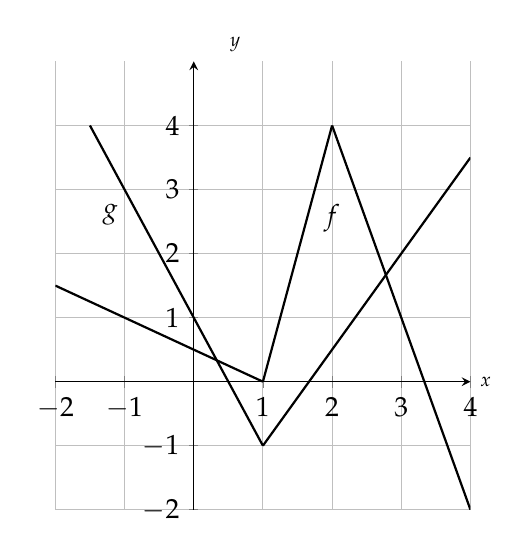
\begin{tikzpicture}
\begin{axis}[axis y line=middle,axis x line=middle, ymajorgrids=true, xmajorgrids=true, ymin=-2,ymax=5, xmin=-2,xmax=4, name=myplot, xscale=1/1.3, ytick={-2,-1,0,1,2,3,4}]
\addplot [{\colorone}, domain=-1.5:1,thick] {-2*x+1}; 
\addplot [{\colorone}, domain=1:4,thick] {1.5*x-2.5};
\addplot [{\colortwo}, domain=-2:1, thick] {-.5*x+.5};
\node[label={30:{$g$}}] at (axis cs:-1.6,2.2) {};
\addplot [{\colortwo}, domain=1:2, thick] {4*x-4};
\node[label={30:{$f$}}] at (axis cs:1.6,2.1) {};
\addplot [{\colortwo}, domain=2:4, thick] {-3*x+10};
\end{axis}
\node [right] at (myplot.right of origin) {\scriptsize $x$};
\node [above] at (myplot.above origin) {\scriptsize $y$};
\end{tikzpicture}
\vskip .5 truecm
You can write this as 4 separately numbered problems, instead of 4 parts of one problem, if it works better that way.\\
(a) $(fg)'(-1)$  \hskip 1 truecm (b) $(f/g)'(-1)$ \hskip 1 truecm (c) $(fg)'(3)$ \hskip 1 truecm (d) $(g/f)'(3)$
\vskip 1 truecm

\textbf{Answers} In the solutions it is fine to list the answer w/o the problem. I just wanted to make sure it was clear which answer went with a problem:\\
\#. $(f + g)'(2)=1$ \\
\#+1. $(f-g)'(2)=-3$\\
\#+2. $(4f)'(2)=-4$ \\
\#+3. $(f \cdot g)'(2)=11$\\
\#+4. $\displaystyle{\left(\frac{f}{g}\right)'(2)=-\frac{1}{25}}$\\ 
\#+5. $\displaystyle{\left(\frac{g}{f+g}\right)'(2) = \frac{1}{4}}$ 
\vskip .5 truecm

Graph problem:\\
(a) $(fg)'(-1)=-\frac{7}{2}$  \vskip .25 truecm 
(b) $(f/g)'(-1)=\frac{1}{8}$ \vskip .25 truecm 
(c) $(fg)'(3) = -\frac{9}{2}$ \vskip .25 truecm 
(d) $(g/f)'(3) = \frac{15}{2}$

%Maybe use this later 3.3 - 41. Find the equation of the tangent line to the graph of $\displaystyle{y = \frac{5}{1+x^2}}$ at each point. \\ (a) $(0, 5)$ \hskip 1 truecm (c) $(-2,1)$  \vskip .5 truecm
%\#. Find the equation of the tangent line to the graph of $y = \text{some product}$ at each point. \\(a) $( ,  )$ \hskip 1 truecm (c) $( , )$  \vskip .5 truecm
%3.3 - 43. Find the $x-$coordinates of all points on the graph of $y=x^3+2x^2-4x+5$ at which the tangent line is (a) horizontal; (b) parallel to the line $2y + 8x - 5 = 0.$\vskip .5 truecm


\newpage


\textbf{Answers} \vskip .25 truecm

20.   Answers vary. Possible solution \\

\begin{tikzpicture}
\begin{axis}[tick label style={font=\scriptsize},minor x tick num=1,axis y line=middle,axis x line=middle,ymin=-3,ymax=2,xmin=-.5,xmax=3.5,name=myplot, xscale=1/1,]
\addplot [domain=-0.5:3.5] {-x*(x-2)};
\end{axis}
\node [right] at (myplot.right of origin) {\scriptsize $x$};
\node [above] at (myplot.above origin) {\scriptsize $y$};
\end{tikzpicture}\\

\vskip .25 truecm

\begin{tikzpicture}
\begin{axis}[tick label style={font=\scriptsize},minor x tick num=1,axis y line=middle,axis x line=middle,ymin=-2,ymax=2,xmin=0,xmax=3,name=myplot, xtick={1,2,3}, xticklabels={1,2,3}, xscale=.6/1,]
\addplot [domain=0:3] {(x-2)^3};
\end{axis}
\node [right] at (myplot.right of origin) {\scriptsize $x$};
\node [above] at (myplot.above origin) {\scriptsize $y$};
\end{tikzpicture}
\vskip 1 truecm



\textbf{Proof: Differentiation Power Rule when $n$ is a positive integer}\vskip .25 truecm
Let $f(x)= x^n$, where $n \in \mathbb{Z}^+$. By the definition of derivative,\\
\small    %%%%%%  Changes text size - makes things fit better.%%%%%%%%%%%
\begin{flalign*}
\begin{aligned}
f'(x) &= \displaystyle{\lim_{h\to 0}} \frac{(x+h)^n - x^n}{h}, ~~\text{where}~ h \neq 0\\
&= \displaystyle{\lim_{h\to 0}} \frac{(x+h)^n - x^n}{h}, ~~\text{use the Binomial Theorem to expand\ } (x+h)^n\\  %%%Changed where this comment is and then there is only one align environment.  
&=\displaystyle{\lim_{h\to 0}} \frac{x^n + \binom{n}{1} hx^{n-1} + \binom{n}{2} h^2x^{n-2}+ ... +\binom{n}{n-1} h^{n-1}x + \binom {n}{n} h^n)   -x^n}{h},\\
&= \displaystyle{\lim_{h\to 0}} \frac{\binom{n}{1} hx^{n-1} + \binom{n}{2} h^2x^{n-2}+ ... +\binom{n}{n-1} h^{n-1}x + \binom {n}{n}  h^n}{h} \\
&= \displaystyle{\lim_{h\to 0}} \frac{\binom{n}{1} hx^{n-1} + \binom{n}{2} h^2x^{n-2}+ ... +\binom{n}{n-1} h^{n-1}x + \binom {n}{n}  h^n}{h} \\
&= \displaystyle{\lim_{h\to 0}} \frac{h[\binom{n}{1} x^{n-1} + \binom{n}{2} h x^{n-2}+ ... +\binom{n}{n-1} h^{n-2}x + \binom {n}{n} h^{n-1}]}{h},~~\text{we divide out}~h\\
&= \displaystyle{\lim_{h\to 0}}~ \binom{n}{1} x^{n-1} + \binom{n}{2} h x^{n-2}+ ... +\binom{n}{n-1} h^{n-2}x + \binom {n}{n} h^{n-1}, ~\text{since} \binom{n}{1} = n \\
&=  n x^{n-1}\\
\end{aligned}
\end{flalign*}
\normalsize  %%%%%Switch back to normal size.

\vskip .5 truecm

Insert proof of Sum Rule\\

\textbf{Proof: Sum Rule for Differentiation}\vskip .25 truecm
Let $f$ and $g$ be differentiable on an open interval $I$ and let $c$ be a real number,\\
\small
\begin{flalign*}
\begin{aligned}
\frac {d}{dx}( f(x) + g(x)) &= \lim_{h\to 0} \frac{[f(x+h)+g(x+h)] - [f(x)+g(x)]}{h}, ~~\text{where}~ h \neq 0\\
&= \lim_{h\to 0} \frac{[f(x+h)-f(x)] + [g(x+h) - g(x)]}{h}\\
&= \lim_{h\to 0} \frac{[f(x+h)-f(x)]}{h} + \lim_{h\to 0}\frac {g(x+h) - g(x)}{h}\\
&= f'(x) + g'(x)\\
\end{aligned}
\end{flalign*}
\normalsize
\vskip .5 truecm


SOLUTION\\
Given the differentiation rules we have thus far, our only option for finding $g'(x)$ is to first multiply $g(x)$ out and then apply the sum and power rules.\\

\begin{center} $g(x) = x^6 + 3x^4 + 3x^2 + 1$ \end{center}
thus, \\
\begin{center}$g'(x) = 6x^5 + 12x^3 + 6x$ \end{center}
\vskip .25 truecm

To differetiate $f(x)$ we will first need to use the Laws of Logarithms to expand $f$. 
\begin{flalign*}
\begin{aligned}
f(x) &= \ln \frac{\sqrt x}{8}\\
 &= \ln x^{\frac{1}{2}} - \ln 8 \\
&= {\frac{1}{2}}\ln x - \ln 8 \\
\end{aligned}
\end{flalign*}
so that,\\
\begin{center} $\displaystyle {f'(x) = {\frac{1}{2}} \cdot \frac{1}{x} -0 = \frac{1}{2x}}$ \end{center} 

\vskip 1.5 truecm


\textbf{p. 84:  Exercises 2.3}
Add the following problems:\\

new \#26 $h(x) = \frac{x^5-2x^3+x^2}{x^2}$\\

new \#27 $f(x) = \frac{x^2+1}{\sqrt x}$\\

new \#28 $g(\theta) = \frac{1-\sin^2 \theta}{\cos \theta}$\\

The current \#26 becomes \#29 then insert the following: \vskip .25 truecm


new\#32 The figure shows the graphs of $f, f', f''$ and $f'''$. Identify each curve and explain your choices.\\

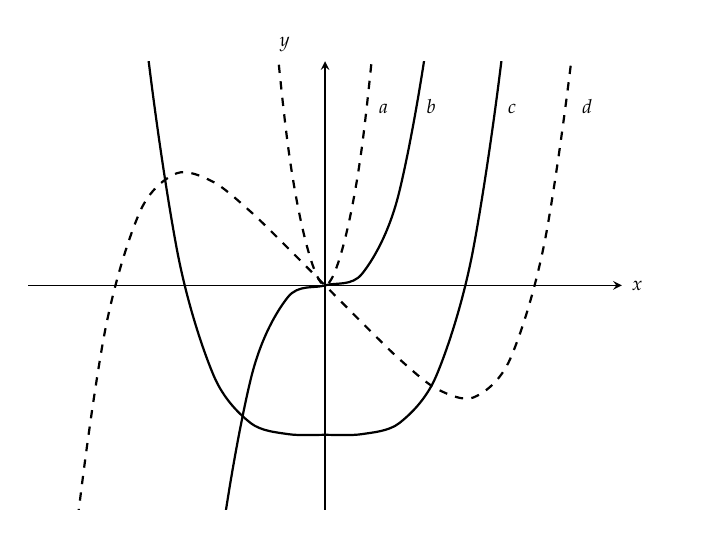
\begin{tikzpicture}
\begin{axis}[xtick=\empty, ytick=\empty, axis y line=middle,axis x line=middle, ymin=-3,ymax=3, xmin=-2,xmax=2, name=myplot, xscale=1.1/1,]
\addplot [{\colorone}, dashed, smooth, domain=-3:3,thick] {.5*x^5-2*x}; 
\node[label={30:{\scriptsize $a$}}] at (axis cs:.23,2.1) {};
\addplot [{\colortwo}, smooth, domain=-3:3,thick] {2.5*x^4-2};
\node[label={30:{\scriptsize $b$}}] at (axis cs:.55,2.1) {};
\addplot [{\colorone}, smooth, domain=-3:3, thick] {10*x^3};
\node[label={30:{\scriptsize $c$}}] at (axis cs:1.1,2.1) {};
\addplot [{\colortwo}, dashed, smooth, domain=-3:3, thick] {30*x^2};
\node[label={30:{\scriptsize $d$}}] at (axis cs:1.6,2.1) {};
\end{axis}
\node [right] at (myplot.right of origin) {\scriptsize $x$};
\node [above] at (myplot.above origin) {\scriptsize $y$};
\end{tikzpicture}
\vskip .5 truecm

The current \#27 - 32 become \#33 - 38 then insert the following: \vskip .25 truecm


new \#39. The position of a object is described by $s(t)=t^4 - 4t^2, t \geq 0$, where $s$ is in feet and $t$ is in seconds. Find\\
(a) the velocity and acceleration functions for the object,\\
(b) the acceleration after 1.5 seconds, and\\
(c) the time, in seconds, the object is at rest.
\vskip .25 truecm


new \#20. Sketch the graph of the function $f$ for which $f(0)=0, f'(0)>0, f'(1)=0,$ and $f'(3)<0$. 

new \#21. Sketch the graph of the function $h$ for which $h(1)=0, h'(1)>0, h'(2)=0,$ and $h'(3)>0$. 



\vskip 1 truecm
\textbf{Answers}\\

26. $h'(x)=3x^2 - 2$\\

27. $f'(x)=\frac{3}{2}\sqrt x  - \frac{1}{2x \sqrt x}$\\ 

28. $g'(\theta)=-\cos \theta$\\ 


30.  $\displaystyle {\frac {d}{dx}(c) = \lim_{h\to 0} \frac{c - c}{h}=0, ~~\text{where}~ h \neq 0}$\vskip .25 truecm

31. $a$ is $f$, $b$ is $f'$, $c$ is $f''$
\vskip .25 truecm

32. $d$ is $f$, $c$ is $f'$, $b$ is $f''$, and $a$ is $f'''$
\vskip .25 truecm

39. (a) $v(t) = 4t^3 - 8t, ~ a(t)=12t^2 - 8$\\
\indent (b) $a(1.5) = 19~ \text{ft/s}^2$\\  
\indent (c) $t=0$ sec and $t=\sqrt{\frac{3}{2}}$ sec
\vskip .25 truecm

40. (a) $v(t) = 5e^x-5, ~ a(t)=5e^x$\\
\indent (b) $a(2) = 5e^2~ \text{ft/s}^2$\\  
\indent (c) $v(t)=0$ at $t=0$ sec, $a(0)=5~ \text{in/s}^2$ 

\end{document}